\documentclass[12pt, onecolumn]{IEEEtran}
\usepackage{cite}
\usepackage{authblk}
\usepackage{amsmath,amssymb,amsfonts}
\usepackage{algorithmic}
\usepackage{graphicx}
\usepackage{textcomp}
\usepackage{xcolor}
\usepackage{hyperref}
\usepackage{booktabs}
\usepackage{float}
\usepackage{svg}
\usepackage{tikz}
\usepackage{pgfplots}
\pgfplotsset{compat=1.18}
\usetikzlibrary{shapes.geometric,arrows.meta,positioning,fit,
             backgrounds,calc,decorations.pathreplacing}

\def\BibTeX{{\rm B\kern-.05em{\sc i\kern-.025em b}\kern-.08em
    T\kern-.1667em\lower.7ex\hbox{E}\kern-.125emX}}

\definecolor{nodeblue}   {RGB}{52,120,210}
\definecolor{nodegray}   {RGB}{200,200,210}
\definecolor{layergreen} {RGB}{34,139,87}
\definecolor{layerpurple}{RGB}{120,60,160}
\definecolor{arrowgray}  {RGB}{110,110,130}
\definecolor{accentorange}{RGB}{230,120,30}
\definecolor{accentred}  {RGB}{200,50,50}
\definecolor{accentgreen}{RGB}{40,160,80}
\definecolor{mqttblue}   {RGB}{0,120,180}
\definecolor{influxpurple}{RGB}{100,50,200}
\definecolor{fastapigreen}{RGB}{0,150,100}
\definecolor{reactcyan}  {RGB}{0,180,210}
\definecolor{edgeorange} {RGB}{220,100,20}
\definecolor{lockred}    {RGB}{210,50,50}
\definecolor{freegreen}  {RGB}{40,160,80}
\definecolor{rewardblue} {RGB}{30,100,200}

\begin{document}

\title{Smart Traffic Signal Control (STC)}

\author[1]{\small Divya Prakash Sinha \texttt{22je0331}}
\author[1]{\small Dyuti Ballav Paul \texttt{22je0335}}
\author[1]{\small Devansh Gupta \texttt{22je0308}}
\author[1]{\small Shreyas Kumar Patel \texttt{22je0925}}
\author[1]{\small Rishit Das \texttt{22je0804}}
\affil[1]{\normalsize Team: D3SR}
\affil[1]{\normalsize Department of Computer Science and Engineering, IIT (ISM) Dhanbad}

\maketitle

\begin{abstract}
Urban traffic congestion remains a critical challenge for smart city infrastructure. Traditional fixed-timing traffic signals fail to adapt to live traffic variability, leading to severe gridlocks and elevated vehicle wait times. This paper details the architecture and implementation of a real-time, adaptive traffic signal control system for a complex urban network (Patna STC, 10 signalized intersections). We propose an architecture combining a Spatial-Temporal Graph Attention Network with Proximal Policy Optimization (STGAT). The model uses 3-head attention with $K{=}3$ hop residual stacking and GRU temporal memory, producing Hold/Switch decisions at 1-second resolution per intersection. Deployed within an IoT-constrained framework, the system leverages SUMO as a Digital Twin simulator, MQTT (Mosquitto) for edge sensor broadcasting, and InfluxDB for time-series persistence. Furthermore, we present an ablation study comparing our GNN approach against Independent Q-Learning and Graph Diffusion Convolution. Our experiments demonstrate a significant reduction in maximum wait times compared to baseline fixed-timing approaches. This document details the architectural approach, physical sensing requirements, engineering challenges resolved, and scalable IoT deployment strategies.
\end{abstract}

\begin{IEEEkeywords}
Reinforcement Learning, Proximal Policy Optimization, Graph Attention Networks, Internet of Things, Traffic Control, Digital Twin, Edge Computing
\end{IEEEkeywords}

\section{Introduction}
Modern urban areas suffer from unpredictable traffic demand, varying vehicle types with disparate passenger car unit (PCU) equivalents, and localized bottlenecks that cause cascading failures across the traffic grid. Pre-timed or actuated traffic signals do not holistically optimize the network state because they lack macroscopic spatial awareness.

With the advent of the Internet of Things (IoT) and deep reinforcement learning (DRL), traffic intersections can now act as intelligent edge devices. By communicating state arrays---such as lane-level queues and signal phases---agents can learn localized optimal switching policies. The core novelty of this paper lies in substituting isolated single-agent reinforcement learning with a \textit{Spatial-Temporal Graph Attention Network (STGAT)}, fused with Proximal Policy Optimization (PPO). This allows a given traffic signal to weight the incoming congestion from neighboring intersections before selfishly maximizing its own throughput. 

\section{Problem Statement and Novelty}
The objective is to minimize intersection wait times and clear dynamic queues across a network of heavily congested intersections in the Patna STC grid. The system must operate at a 1-second resolution, broadcasting metrics and applying phase-switch decisions in soft real-time.

\subsection{What makes this challenging in Real-World Scenarios?}
\begin{itemize}
    \item \textbf{Non-Stationarity:} Traffic flow shifts dramatically due to peak hours, rendering deterministic models ineffective.
    \item \textbf{Heterogeneous Traffic:} Traffic in dense regions is highly mixed (motorcycles, auto-rickshaws, buses) requiring unified Passenger Car Unit (PCU) proxy metrics.
    \item \textbf{Ripple Effects:} A delayed green light at Node A quickly blocks the outflow of Node B. Greedy local optimization often worsens global gridlock.
    \item \textbf{Soft Real-Time Constraint:} The full pipeline---sensor ingestion, GNN forward pass, and PLC command dispatch---must complete within 1 second per tick.
\end{itemize}

\subsection{Formal Problem Definition}
We model the traffic network as a directed graph $\mathcal{G} = (\mathcal{V}, \mathcal{E}, A)$ where $\mathcal{V} = \{v_1, \ldots, v_N\}$ represents $N=10$ signalized intersections, $\mathcal{E}$ represents physical road connections, and $A \in \mathbb{R}^{N \times N}$ is a weighted adjacency matrix with:
\begin{equation}
    A_{ij} = \begin{cases}
        \frac{100}{d_{\text{BFS}}(v_i, v_j) + 1} & \text{if } v_j \text{ reachable from } v_i \\
        100 & \text{if } i = j \; (\text{self-loop}) \\
        0 & \text{otherwise}
    \end{cases}
\end{equation}
where $d_{\text{BFS}}(v_i, v_j)$ is the accumulated road length from a BFS traversal that skips unsignalized nodes.

At each discrete time step $t$, each intersection $v_i$ observes a local state vector:
\begin{equation}
    \mathbf{s}_i^{(t)} = \left[ \frac{q_i^{(t)}}{50}, \; \frac{w_i^{(t)}}{100}, \; \frac{\phi_i^{(t)}}{|\Phi_i|}, \; \min\!\left(\frac{\tau_i^{(t)}}{15}, 1\right) \right] \in \mathbb{R}^4
\end{equation}
where $q_i$ is the PCU-weighted queue length, $w_i$ is the maximum accumulated wait time (seconds), $\phi_i$ is the current phase index, $|\Phi_i|$ is the total number of phases, and $\tau_i$ is the time elapsed since the last phase change.

The agent selects a binary action $a_i^{(t)} \in \{0, 1\}$ (Hold/Switch) for each intersection. The per-node reward is:
\begin{equation}
    r_i^{(t)} = -\left( q_i^{(t)} + \omega \cdot w_i^{(t)} \right) - \mathbb{1}[a_i^{(t)} = 1] \cdot \lambda_{\text{switch}}
\end{equation}
where $\omega = 0.5$ balances queue vs.\ wait importance, and $\lambda_{\text{switch}} = 15.0$ penalizes excessive phase cycling. The global step reward is $R^{(t)} = \sum_{i=1}^{N} r_i^{(t)}$.

\subsection{The Novelty of STGAT in Traffic Flow}
Traditional Reinforcement Learning (RL) forces agents to learn the state of the entire map as a flattened vector map, which breaks down if the map topology changes or scales up. Our STGAT approach treats the traffic grid as a localized Graph:
\begin{itemize}
 \item \textbf{Attention Mechanism:} By using multiple attention heads, an intersection can dynamically ``pay attention'' to a $K$-hop neighbor. If Node B has an overflowing queue headed toward Node A, Node A's attention weights shift, prompting it to alter its phase to accommodate the incoming surge.
    \item \textbf{Shift from Independent Learning:} Independent actors behave selfishly. STGAT forces mathematical collaboration without requiring centralized brute-force computation.

    \begin{figure}[H]
    \centering
    % \includegraphics[width=0.95\linewidth]{stgat_architecture.png}
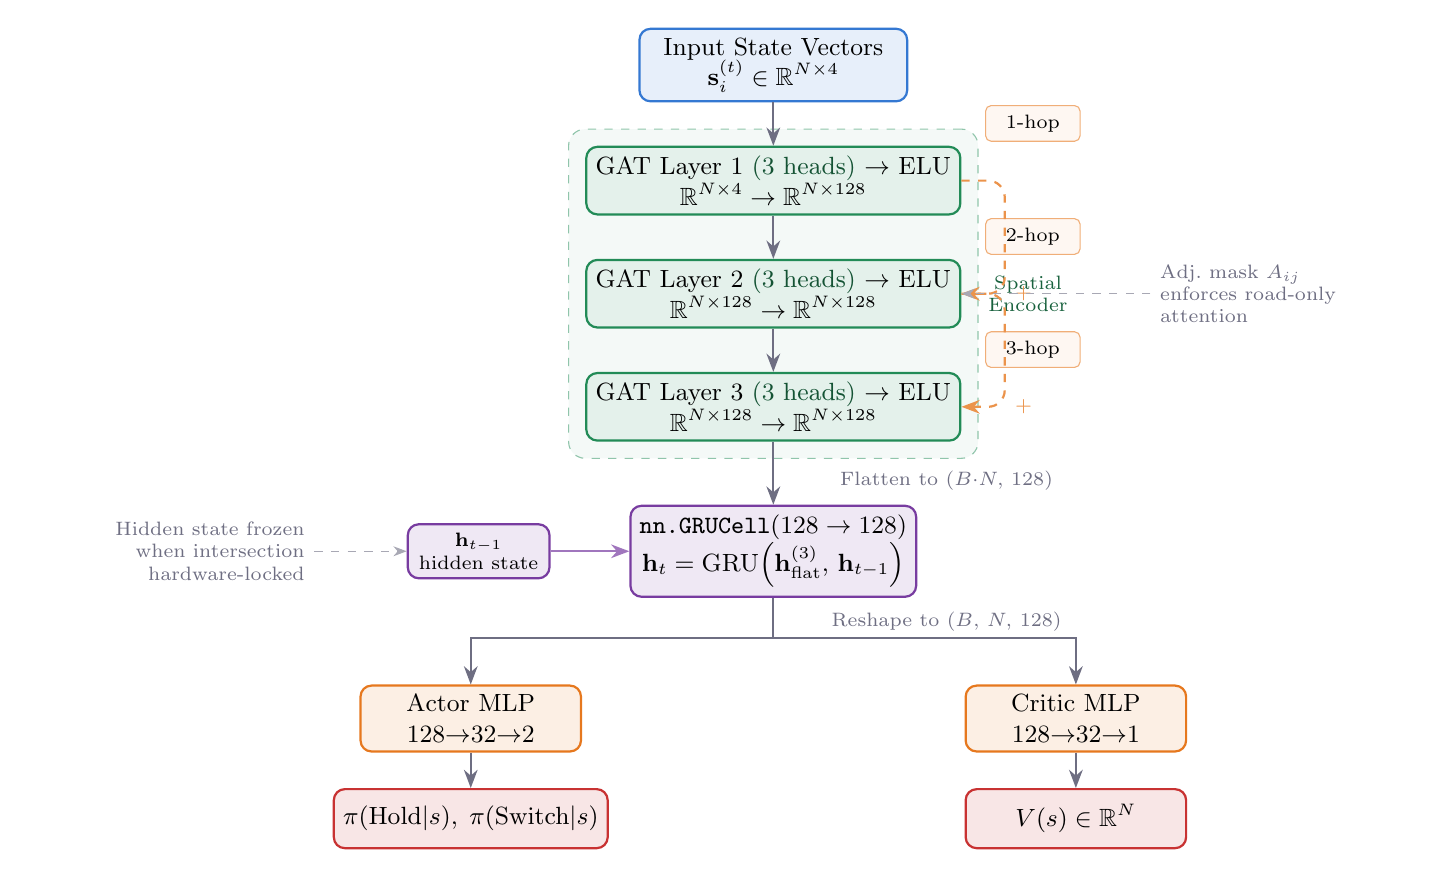
\begin{tikzpicture}[
  font=\small,
  >=Stealth,
  every node/.style={align=center},
  inpbox/.style={rectangle, rounded corners=4pt,
    draw=nodeblue, fill=nodeblue!12,
    minimum width=3.4cm, minimum height=0.75cm, line width=0.8pt},
  gatbox/.style={rectangle, rounded corners=4pt,
    draw=layergreen, fill=layergreen!12,
    minimum width=3.4cm, minimum height=0.85cm, line width=0.8pt},
  grubox/.style={rectangle, rounded corners=4pt,
    draw=layerpurple, fill=layerpurple!12,
    minimum width=3.4cm, minimum height=0.85cm, line width=0.8pt},
  actbox/.style={rectangle, rounded corners=4pt,
    draw=accentorange, fill=accentorange!12,
    minimum width=2.8cm, minimum height=0.75cm, line width=0.8pt},
  outbox/.style={rectangle, rounded corners=4pt,
    draw=accentred, fill=accentred!12,
    minimum width=2.8cm, minimum height=0.75cm, line width=0.8pt},
  resbox/.style={rectangle, rounded corners=2pt,
    draw=accentorange!60, fill=accentorange!6,
    minimum width=1.2cm, minimum height=0.4cm, font=\scriptsize},
  arr/.style={->, thick, color=arrowgray},
  reskip/.style={->, thick, dashed, color=accentorange!80, rounded corners=6pt},
]
 
% Input
\node[inpbox] (inp) {Input State Vectors\\$\mathbf{s}_i^{(t)} \in \mathbb{R}^{N \times 4}$};
 
% GAT Layer 1
\node[gatbox, below=0.55cm of inp] (gat1)
  {GAT Layer 1 \textcolor{layergreen!60!black}{(3 heads)} $\to$ ELU\\
   $\mathbb{R}^{N\times 4} \to \mathbb{R}^{N\times 128}$};
\node[resbox, above right=0.05cm and 0.3cm of gat1] {1-hop};
 
% GAT Layer 2
\node[gatbox, below=0.55cm of gat1] (gat2)
  {GAT Layer 2 \textcolor{layergreen!60!black}{(3 heads)} $\to$ ELU\\
   $\mathbb{R}^{N\times 128} \to \mathbb{R}^{N\times 128}$};
\node[resbox, above right=0.05cm and 0.3cm of gat2] {2-hop};
 
% GAT Layer 3
\node[gatbox, below=0.55cm of gat2] (gat3)
  {GAT Layer 3 \textcolor{layergreen!60!black}{(3 heads)} $\to$ ELU\\
   $\mathbb{R}^{N\times 128} \to \mathbb{R}^{N\times 128}$};
\node[resbox, above right=0.05cm and 0.3cm of gat3] {3-hop};
 
% Flatten annotation
\node[font=\scriptsize, text=arrowgray, below=0.25cm of gat3, xshift=2.2cm] (flatnote)
  {Flatten to $(B{\cdot}N,\,128)$};
 
% GRU
\node[grubox, below=0.80cm of gat3] (gru)
  {\texttt{nn.GRUCell}$(128 \to 128)$\\
   $\mathbf{h}_t = \text{GRU}\!\left(\mathbf{h}^{(3)}_\text{flat},\,\mathbf{h}_{t-1}\right)$};
 
% Reshape annotation
\node[font=\scriptsize, text=arrowgray, below=0.05cm of gru, xshift=2.2cm] (reshapnote)
  {Reshape to $(B,\,N,\,128)$};
 
% Previous hidden state
\node[grubox, left=1.0cm of gru,
      minimum width=1.8cm, minimum height=0.6cm, font=\scriptsize] (hprev)
  {$\mathbf{h}_{t-1}$\\hidden state};
\draw[arr, color=layerpurple!70] (hprev) -- (gru);
 
% Actor / Critic
\node[actbox, below left=1.10cm and 0.6cm of gru]  (actor)  {Actor MLP\\$128{\to}32{\to}2$};
\node[actbox, below right=1.10cm and 0.6cm of gru] (critic) {Critic MLP\\$128{\to}32{\to}1$};
 
% Outputs
\node[outbox, below=0.45cm of actor]
  (policy) {$\pi(\text{Hold}|s),\;\pi(\text{Switch}|s)$};
\node[outbox, below=0.45cm of critic]
  (value)  {$V(s) \in \mathbb{R}^N$};
 
% Main arrows
\draw[arr] (inp)  -- (gat1);
\draw[arr] (gat1) -- (gat2);
\draw[arr] (gat2) -- (gat3);
\draw[arr] (gat3) -- (gru);
\draw[arr] (gru)  -- ++(0, -1.10) -| (actor);
\draw[arr] (gru)  -- ++(0, -1.10) -| (critic);
\draw[arr] (actor)  -- (policy);
\draw[arr] (critic) -- (value);
 
% Residual skip connections
\draw[reskip] (gat1.east) -- ++(0.55,0) |- (gat2.east)
  node[midway, right, font=\scriptsize, color=accentorange!80]{$+$};
\draw[reskip] (gat2.east) -- ++(0.55,0) |- (gat3.east)
  node[midway, right, font=\scriptsize, color=accentorange!80]{$+$};
 
% Adjacency mask note
\node[right=2.4cm of gat2, font=\scriptsize, text=arrowgray,
      text width=3cm, align=left] (note)
  {Adj.\ mask $A_{ij}$\\enforces road-only\\attention};
\draw[->, dashed, color=arrowgray!60, thin] (note.west) -- (gat2.east);
 
% GRU frozen note
\node[left=4.0cm of gru, font=\scriptsize, text=arrowgray,
      text width=3.4cm, align=right] (grunote)
  {Hidden state frozen\\when intersection\\hardware-locked};
\draw[->, dashed, color=arrowgray!60, thin] (grunote.east) -- (hprev.west);
 
% Spatial encoder bounding box
\begin{scope}[on background layer]
  \node[draw=layergreen!50, fill=layergreen!5, rounded corners=6pt,
        dashed, inner sep=6pt,
        fit=(gat1)(gat2)(gat3),
        label={[font=\scriptsize\color{layergreen!70!black}]right:Spatial\\Encoder}] {};
\end{scope}
\end{tikzpicture}
    \caption{STGAT model architecture: Multi-Head Graph Attention layers with $K$-hop residual stacking feeding into a GRU temporal memory unit, producing per-intersection Hold/Switch action probabilities through an Actor-Critic head.}
    \label{fig:stgat_arch}
    \end{figure}
\end{itemize}

\section{STGAT Architecture: Detailed Walkthrough}

This section provides a layer-by-layer explanation of the Spatial-Temporal Graph Attention Network as implemented in our codebase. The model (\texttt{STGAT\_ActorCritic}) uses \texttt{feature\_dim=4}, \texttt{hidden\_dim=128}, \texttt{num\_actions=2} (Hold/Switch), \texttt{k\_hops=3}, and \texttt{num\_heads=3}. We justify the architectural choices against alternatives such as full Transformers.

\subsection{Why Not a Full Transformer?}
A full Transformer (e.g., GPT, BERT) applies self-attention over a flat sequence of tokens, allowing every token to attend to every other token. While powerful for natural language, this design is fundamentally misaligned with traffic networks for three reasons:
\begin{enumerate}
    \item \textbf{Topology Ignorance:} A Transformer would allow Intersection 1 to attend to Intersection 10 even if no physical road connects them. Our GAT layer masks attention using the adjacency matrix $A$, ensuring information flows only along real roads.
    \item \textbf{Computational Overhead:} Full self-attention is $O(N^2)$ across all node pairs. Our adjacency-masked GAT is effectively $O(|E|)$ where $|E|$ is the number of edges (roads), which is significantly sparser.
    \item \textbf{Redundant Mechanism:} The core innovation of the Transformer is multi-head attention --- and we already incorporate it. Our architecture extracts the ``secret sauce'' of Transformers (multi-head attention) while constraining it to the physical graph topology, which is more principled for spatial infrastructure networks.
\end{enumerate}

\subsection{Multi-Head Graph Attention Layer (GATLayer)}
Each GATLayer performs the following operations:

\subsubsection{Step 1: Feature Projection into Multiple Heads}
Each intersection's 4-dimensional feature vector $\mathbf{x}_i = [\text{queue}_{\text{pcu}}/50, \; \text{max\_wait}/100, \; \text{phase}/N_{\text{phases}}, \; \min(t_{\text{elapsed}}/15, 1)]$ is projected into $H=3$ separate subspaces via a shared linear transformation $\mathbf{W} \in \mathbb{R}^{4 \times (128 \cdot 3)}$ (without bias):
\begin{equation}
    \mathbf{W}\mathbf{h}_i = \text{Linear}(\mathbf{x}_i) \in \mathbb{R}^{H \times d_{\text{hidden}}}
\end{equation}
Each head learns a \textit{different perspective} of the traffic state. Intuitively:
\begin{itemize}
    \item \textbf{Head 1} may specialize in detecting \textit{queue pressure} from neighbors.
    \item \textbf{Head 2} may focus on \textit{phase synchronization} patterns.
    \item \textbf{Head 3} may track \textit{wait-time urgency} signals.
\end{itemize}

\subsubsection{Step 2: Attention Scoring}
For each head, the model computes pairwise attention coefficients between connected intersections using separate learnable source and destination vectors $\mathbf{a}_{src}$ and $\mathbf{a}_{dst}$:
\begin{equation}
    e_{ij}^{(h)} = \text{LeakyReLU}\left( \mathbf{a}_{src}^{(h)\top} \mathbf{W}\mathbf{h}_i + \mathbf{a}_{dst}^{(h)\top} \mathbf{W}\mathbf{h}_j \right)
\end{equation}
This score answers: \textit{``How much should Node $i$ care about Node $j$'s traffic state right now?''}

\subsubsection{Step 3: Adjacency Masking (GNN vs. Transformer)}
This is the critical architectural distinction. Attention scores for non-connected intersections are masked to $-\infty$:
\begin{equation}
    \alpha_{ij}^{(h)} = \begin{cases}
        \text{softmax}_j(e_{ij}^{(h)}) & \text{if } A_{ij} > 0 \\
        0 & \text{otherwise}
    \end{cases}
\end{equation}
Only physically connected road neighbors can influence each other. A full Transformer omits this step entirely, allowing unconstrained all-to-all attention.

\subsubsection{Step 4: Head Aggregation}
The outputs of all $H$ heads are averaged back into a single $d_{out}$-dimensional vector per node:
\begin{equation}
    \mathbf{h}'_i = \text{ELU}\left( \frac{1}{H} \sum_{h=1}^{H} \sum_{j \in \mathcal{N}(i)} \alpha_{ij}^{(h)} \mathbf{W}^{(h)} \mathbf{h}_j \right)
\end{equation}

\subsection{Multi-Hop Stacking with Residual Connections}
We stack $K=3$ GATLayers sequentially (one \texttt{ModuleList} of \texttt{GATLayer} instances). The first layer maps the 4D input to 128D. After layer 1, each node aggregates information from its direct (1-hop) neighbors. After layer 2, it has indirect awareness of 2-hop neighbors. After layer 3, information has diffused across the 3-hop spatial receptive field.

Crucially, layers 2 and 3 use \textbf{residual connections} (additive skip connections):
\begin{equation}
    \mathbf{h}^{(k+1)} = \mathbf{h}^{(k)} + \text{GAT}^{(k+1)}(\mathbf{h}^{(k)}, A) \qquad \text{for } k = 1, 2
\end{equation}
This prevents gradient degradation in deeper layers and allows the model to preserve local features while enriching them with neighborhood context.

Note: the adjacency matrix $A$ includes weighted self-loops ($A_{ii} = 100$) and edge weights computed as $100 / (d_{\text{road}} + 1)$ where $d_{\text{road}}$ is the BFS-accumulated road distance between signalized intersections.

\begin{figure}[H]
\centering
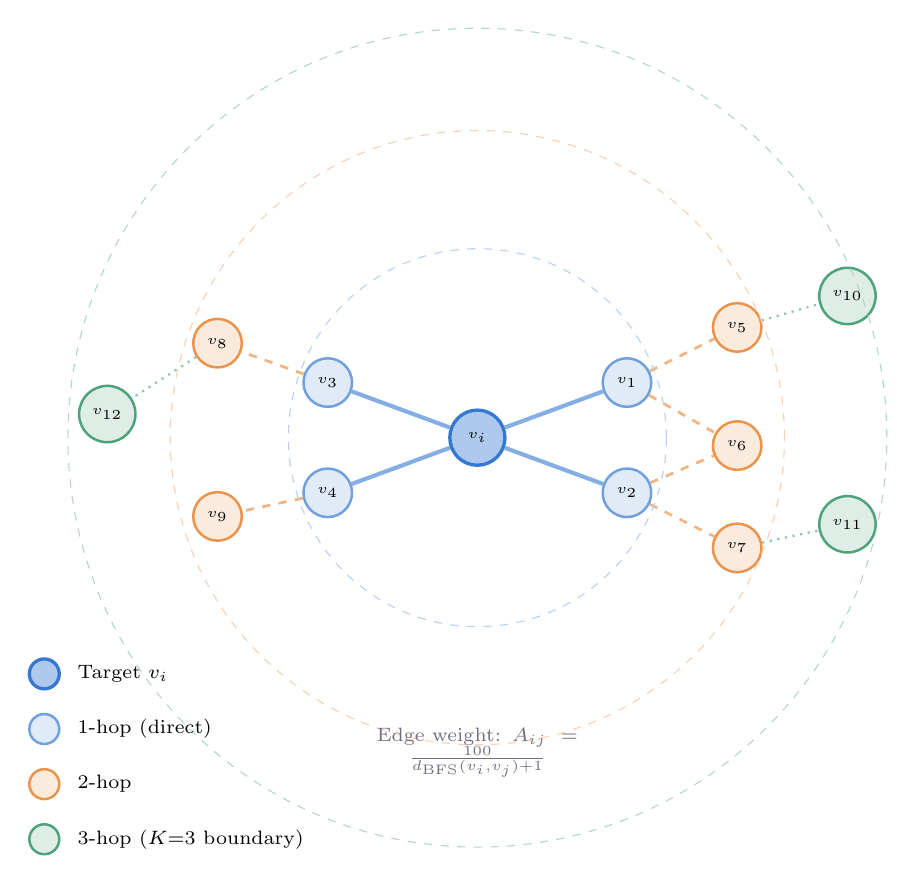
\begin{tikzpicture}[
  font=\small, >=Stealth,
  node0/.style={circle, draw=nodeblue,     fill=nodeblue!40,
                minimum size=0.70cm, line width=1.2pt},
  node1/.style={circle, draw=nodeblue!70,  fill=nodeblue!15,
                minimum size=0.60cm, line width=0.9pt},
  node2/.style={circle, draw=accentorange!80, fill=accentorange!15,
                minimum size=0.55cm, line width=0.9pt},
  node3/.style={circle, draw=layergreen!80, fill=layergreen!15,
                minimum size=0.50cm, line width=0.9pt},
  e1/.style={draw=nodeblue!60,     line width=1.5pt},
  e2/.style={draw=accentorange!55, line width=1.0pt, dashed},
  e3/.style={draw=layergreen!50,   line width=0.8pt, dotted},
]
 
% Centre
\node[node0] (c) at (0,0) {\tiny$v_i$};
 
% 1-hop
\node[node1] (h1a) at ( 1.9,  0.7) {\tiny$v_1$};
\node[node1] (h1b) at ( 1.9, -0.7) {\tiny$v_2$};
\node[node1] (h1c) at (-1.9,  0.7) {\tiny$v_3$};
\node[node1] (h1d) at (-1.9, -0.7) {\tiny$v_4$};
 
% 2-hop
\node[node2] (h2a) at ( 3.3,  1.4) {\tiny$v_5$};
\node[node2] (h2b) at ( 3.3, -0.1) {\tiny$v_6$};
\node[node2] (h2c) at ( 3.3, -1.4) {\tiny$v_7$};
\node[node2] (h2d) at (-3.3,  1.2) {\tiny$v_8$};
\node[node2] (h2e) at (-3.3, -1.0) {\tiny$v_9$};
 
% 3-hop
\node[node3] (h3a) at ( 4.7,  1.8) {\tiny$v_{10}$};
\node[node3] (h3b) at ( 4.7, -1.1) {\tiny$v_{11}$};
\node[node3] (h3c) at (-4.7,  0.3) {\tiny$v_{12}$};
 
% Edges
\draw[e1] (c)--(h1a); \draw[e1] (c)--(h1b);
\draw[e1] (c)--(h1c); \draw[e1] (c)--(h1d);
\draw[e2] (h1a)--(h2a); \draw[e2] (h1a)--(h2b);
\draw[e2] (h1b)--(h2b); \draw[e2] (h1b)--(h2c);
\draw[e2] (h1c)--(h2d); \draw[e2] (h1d)--(h2e);
\draw[e3] (h2a)--(h3a); \draw[e3] (h2c)--(h3b);
\draw[e3] (h2d)--(h3c);
 
% Concentric rings
\draw[nodeblue!35,     dashed, thin] (0,0) circle (2.4cm);
\draw[accentorange!35, dashed, thin] (0,0) circle (3.9cm);
\draw[layergreen!35,   dashed, thin] (0,0) circle (5.2cm);
 
% Legend (bottom left)
\node[node0, minimum size=0.38cm] at (-5.5, -3.0) {};
\node[right, font=\scriptsize] at (-5.2,-3.0) {Target $v_i$};
\node[node1, minimum size=0.38cm] at (-5.5, -3.7) {};
\node[right, font=\scriptsize] at (-5.2,-3.7) {1-hop (direct)};
\node[node2, minimum size=0.38cm] at (-5.5, -4.4) {};
\node[right, font=\scriptsize] at (-5.2,-4.4) {2-hop};
\node[node3, minimum size=0.38cm] at (-5.5, -5.1) {};
\node[right, font=\scriptsize] at (-5.2,-5.1) {3-hop ($K{=}3$ boundary)};
 
\node[font=\scriptsize, color=arrowgray, text width=4cm, align=center]
  at (0,-4.0) {Edge weight: $A_{ij}=\frac{100}{d_\mathrm{BFS}(v_i,v_j)+1}$};
 
\end{tikzpicture}
\caption{$K$-hop spatial receptive field (illustrative; actual Patna STC has $N{=}10$). After $K{=}3$ GAT layers,
a target intersection has aggregated spatial information from all
intersections within 3 road-hops. BFS-weighted edges ensure only
physically connected nodes exchange information.}
\label{fig:khop}
\end{figure}

\subsection{Temporal Memory via GRU}
The spatially enriched features are fed into a standard \texttt{nn.GRUCell} (128$\to$128) that maintains a hidden state $\mathbf{h}_{t-1}$ from the previous simulation second. During inference, the spatial feature tensor is flattened to $(B{\cdot}N, 128)$, processed through the GRU, then reshaped back to $(B, N, 128)$:
\begin{equation}
    \mathbf{h}_t = \text{GRUCell}(\mathbf{h}^{(K)}_{\text{spatial}}, \mathbf{h}_{t-1})
\end{equation}
This gives the model a temporal memory of how traffic \textit{evolves} over time. Importantly, during asynchronous inference, when an intersection is hardware-locked (executing a yellow$\to$green transition), its GRU hidden state is \textit{frozen} (not updated) until the lock expires, preventing temporal corruption.

\subsection{Actor-Critic Heads}
The GRU output feeds two separate MLPs:
\begin{itemize}
    \item \textbf{Actor:} $\text{Linear}(128 \to 32) \to \text{ReLU} \to \text{Linear}(32 \to 2) \to \text{Softmax}$ — producing per-node action probabilities $\pi(\text{Hold} | s)$ and $\pi(\text{Switch} | s)$.
    \item \textbf{Critic:} $\text{Linear}(128 \to 32) \to \text{ReLU} \to \text{Linear}(32 \to 1)$ — producing per-node state value estimates $V(s)$.
\end{itemize}
Both heads use orthogonal initialization following the OpenAI PPO standard.

\subsection{PPO Training Objective}
The model is trained using the Proximal Policy Optimization (PPO-Clip) algorithm. For each collected trajectory, we compute the Generalized Advantage Estimate (GAE) and optimize the clipped surrogate objective.

Let $\pi_{\theta}$ denote the current policy and $\pi_{\theta_{\text{old}}}$ the policy used to collect the trajectory. The probability ratio is:
\begin{equation}
    \rho_t = \frac{\pi_{\theta}(a_t | s_t)}{\pi_{\theta_{\text{old}}}(a_t | s_t)}
\end{equation}

The clipped surrogate loss prevents destructively large policy updates:
\begin{equation}
    \mathcal{L}^{\text{CLIP}} = -\mathbb{E}_t \left[ \min\!\left( \rho_t \hat{A}_t, \; \text{clip}(\rho_t, 1{-}\epsilon, 1{+}\epsilon) \hat{A}_t \right) \right]
\end{equation}
where $\hat{A}_t$ is the advantage estimate and $\epsilon$ is the clipping threshold (typically 0.2).

The critic is trained with a standard value function loss:
\begin{equation}
    \mathcal{L}^{\text{VF}} = \mathbb{E}_t \left[ \left( V_{\theta}(s_t) - V^{\text{target}}_t \right)^2 \right]
\end{equation}

An entropy bonus $\mathcal{H}[\pi_{\theta}]$ is added to encourage exploration. The combined loss is:
\begin{equation}
    \mathcal{L} = \mathcal{L}^{\text{CLIP}} + c_1 \mathcal{L}^{\text{VF}} - c_2 \mathcal{H}[\pi_{\theta}]
\end{equation}
where $c_1$ and $c_2$ are hyperparameter coefficients.

The \texttt{evaluate()} function in the model re-runs the full spatial-temporal pipeline (GAT $\to$ GRU $\to$ Actor/Critic) on buffered states to compute fresh log-probabilities, value estimates, and entropy for each PPO epoch.

\subsection{Comparative Summary}
Table~\ref{tab:transformer_comparison} summarizes the architectural comparison:

\begin{table}[H]
\centering
\caption{Architectural Comparison: Full Transformer vs. STGAT}
\label{tab:transformer_comparison}
\resizebox{0.8\linewidth}{!}{
\begin{tabular}{@{}lcc@{}}
\toprule
\textbf{Aspect} & \textbf{Full Transformer} & \textbf{Our STGAT} \\
\midrule
Attention scope       & All-to-all (wasteful)   & Road-constrained  \\
Multi-head attention  & \checkmark              & \checkmark (3 heads) \\
Topology-aware        & $\times$                & \checkmark (adj mask) \\
Temporal memory       & Positional enc. (static) & GRU (dynamic recurrent) \\
Scalability           & $O(N^2)$ full           & $O(|E|)$ sparse \\
Residual connections  & \checkmark              & \checkmark ($K$-hop) \\
Edge-deployable       & $\times$ (heavy)        & \checkmark (lightweight) \\
\bottomrule
\end{tabular}
}
\end{table}


\section{System Architecture and Physical Translation}

The system features a microservices architecture bifurcated into Edge Inference, Cloud Infrastructure, and a live Dashboard UI. Figure \ref{fig:architecture} illustrates the high-level topology.

\begin{figure}[H]
    \centering
    \resizebox{\linewidth}{!}{
    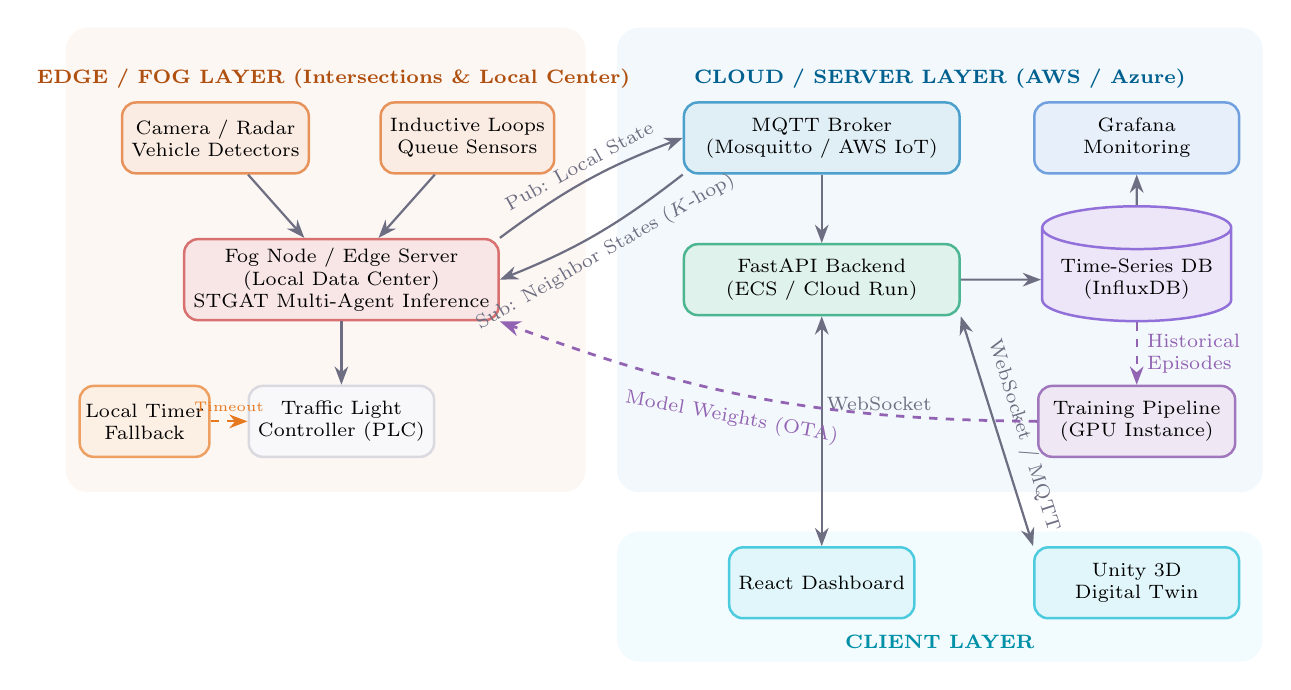
\begin{tikzpicture}[
      font=\scriptsize, >=Stealth,
      every node/.style={align=center},
      compbox/.style={rectangle, rounded corners=5pt,
        draw=#1!70, fill=#1!12,
        minimum width=2.6cm, minimum height=0.9cm, line width=0.9pt},
      db/.style={cylinder, draw=#1!70, fill=#1!12, shape border rotate=90, aspect=0.25,
        minimum width=2.4cm, minimum height=1.1cm, line width=0.9pt},
      arr/.style={->, thick, color=arrowgray},
      darr/.style={<->, thick, color=arrowgray},
    ]
     
    % ── EDGE LAYER ──────────────────────────────────────────────
    \node[compbox=edgeorange, minimum width=1.5] (cam) at (-4.5, 1.8) {Camera / Radar\\Vehicle Detectors};
    \node[compbox=edgeorange, minimum width=1.5] (loop) at (-1.3, 1.8) {Inductive Loops\\Queue Sensors};
     
    \node[compbox=accentred, minimum width=2.5cm] (edge) at (-2.9, 0)
      {Fog Node / Edge Server\\(Local Data Center)\\STGAT Multi-Agent Inference};
     
    \node[compbox=nodegray, minimum width=1.9cm] (plc) at (-2.9, -1.8) {Traffic Light\\Controller (PLC)};
    \node[compbox=accentorange, minimum width=1.4cm, font=\scriptsize, inner sep=2pt] (fallback) at (-5.4, -1.8) {Local Timer\\Fallback};
     
    \draw[arr] (cam) -- (edge);
    \draw[arr] (loop) -- (edge);
    \draw[arr] (edge) -- (plc);
    \draw[arr, dashed, color=accentorange] (fallback) -- node[above, font=\tiny]{Timeout} (plc);
     
    % ── CLOUD LAYER ─────────────────────────────────────────────
    \node[compbox=mqttblue, minimum width=3.5cm] (mqtt) at (3.2, 1.8)
      {MQTT Broker\\(Mosquitto / AWS IoT)};
     
    \node[compbox=fastapigreen, minimum width=3.5cm] (api) at (3.2, 0)
      {FastAPI Backend\\(ECS / Cloud Run)};
     
    \node[db=influxpurple] (tsdb) at (7.2, 0) {Time-Series DB\\(InfluxDB)};
     
    \node[compbox=nodeblue] (grafana) at (7.2, 1.8) {Grafana\\Monitoring};
     
    \node[compbox=layerpurple, minimum width=2.5cm] (train) at (7.2, -1.8)
      {Training Pipeline\\(GPU Instance)};
     
    \draw[arr] (mqtt) -- (api);
    \draw[arr] (api) -- (tsdb);
    \draw[arr] (tsdb) -- (grafana);
    \draw[arr, dashed, color=layerpurple!80] (tsdb.south) -- node[right, font=\scriptsize, align=left]{Historical\\Episodes} (train.north);
     
    % ── CLIENT LAYER ────────────────────────────────────────────
    \node[compbox=reactcyan, minimum width=2.5] (dash) at (3.2, -3.85) {React Dashboard};
    \node[compbox=reactcyan] (mobile) at (7.2, -3.85) {Unity 3D\\Digital Twin};
     
    \draw[arr, <->] (api) -- node[right, yshift=10pt, xshift=-2pt, font=\scriptsize]{WebSocket} (dash);
    \draw[arr, <->] (api.south east) -- node[above=0.05cm, sloped, font=\scriptsize, pos=0.55]{WebSocket / MQTT} (mobile.north west);
     
    % ── CROSS-LAYER CONNECTIONS ─────────────────────────────────
    \draw[arr] (edge.north east) to[bend left=8]
      node[above, sloped, font=\scriptsize]{Pub: Local State} (mqtt.west);

    \draw[arr] (mqtt.south west) to[bend left=8]
      node[below, sloped, font=\scriptsize]{Sub: Neighbor States ($K$-hop)} (edge.east);
      
    \draw[arr, dashed, color=layerpurple!80, line width=1pt] (train.west) to[bend left=10] 
      node[below=0.05cm, xshift=-10pt, sloped, font=\scriptsize]{Model Weights (OTA)} (edge.south east);
     
    % ── Layer bands ─────────────────────────────────────────────
    \begin{scope}[on background layer]
    \fill[edgeorange!5, rounded corners=8pt] (-6.4, 3.2) rectangle (0.2,-2.7);
    \fill[mqttblue!5, rounded corners=8pt] (0.6, 3.2) rectangle (8.8,-2.7);
    \fill[reactcyan!5, rounded corners=8pt] (0.6, -3.2) rectangle (8.8,-4.85);
     
    \node[font=\bfseries\scriptsize, color=edgeorange!80!black] at (-3.0, 2.55) {EDGE / FOG LAYER (Intersections \& Local Center)};
    \node[font=\bfseries\scriptsize, color=mqttblue!80!black]   at (4.7, 2.55) {CLOUD / SERVER LAYER (AWS / Azure)};
    \node[font=\bfseries\scriptsize, color=reactcyan!80!black]  at (4.7, -4.6) {CLIENT LAYER};
    \end{scope}
     
    \end{tikzpicture}
    }
    \caption{Proposed IoT Architecture for Real-World Deployment encompassing Edge Sensors, Cloud Aggregation (MQTT/TSDB), GPU Training Pipeline, and Client Dashboard interfaces.}
    \label{fig:architecture}
\end{figure}

\subsection{Real-World Implementation and Fog Computing Mapping}
Translating the SUMO Digital Twin into a physical deployment requires robust sensing arrays and edge-centralized intelligence.
\begin{enumerate}
    \item \textbf{Cameras and Local Feature Extraction:} Pole-mounted CCTV arrays stream video to lightweight municipal access points running YOLOv8 object detection to count vehicles per lane and classify them into PCU types (Car=1.0, Bus=3.0, Tracker=0.5).
    \item \textbf{Phase State Sensors:} Dedicated PLCs connected to physical traffic signal cabinets relay the \textit{Current Phase} to the Fog Node.
    \item \textbf{Fog Computing Pipeline:} Rather than placing an expensive Deep Learning PC at every intersection that relies on localized neighbor broadcasts, a centralized Municipal Edge Server (\textit{Fog Node}) aggregates the $[Queue, Wait, Phase]$ tensors from all intersections in a unified hub. It constructs the holistic spatial graph instantaneously, executes the STGAT forward pass, and dispatches coordinated \textit{Hold/Switch} commands back to the individual intersection PLCs.
    \item \textbf{Safety Fallback Mechanism:} In cases of network dropout where Fog connectivity fails, local Traffic PLCs utilize a hardware-level timeout to revert to a fixed-cycle signal plan, safely guaranteeing infrastructural stability.
\end{enumerate}

\subsection{IoT Protocol and Data Backbone}
To simulate this reality, our backend relies on:
\begin{itemize}
    \item \textbf{MQTT Broker (Mosquitto):} Edge metrics are published to \texttt{stc/traffic/sensors}.
    \item \textbf{Time-Series DB (InfluxDB):} The telemetry is asynchronously serialized for historical training loops and visualizations.
    \item \textbf{FastAPI WebSockets:} A high-frequency layer pushing the raw tensors directly to the React frontend.
    \item \textbf{Unity 3D Engine:} A photorealistic 3D visualization layer consuming live coordinate telemetry to render a high-fidelity spatial Digital Twin of the intersection network.
\end{itemize}

\section{Ablation and Comparative Study}

To empirically justify the architecture, we evaluated the STGAT approach against several alternatives in our Digital Twin environment.

\subsection{Independent Q-Learning (IQL) vs. GNN}
\paragraph{Approach} We initially tested Independent Q-Learning, where each intersection hosted its own isolated DQN actor. \\
\paragraph{Drawback} IQL agents rapidly minimized their immediate queues by turning lights green, oblivious to the fact that they were discharging traffic into an already-full downstream adjacent intersection. This caused severe "grid-locking" where lanes became physically blocked, preventing geometric movement. \\
\paragraph{The GNN Advantage} The Graph Attention layer prevented this by allowing intersections to sense downstream blockages up to $K=3$ hops away, naturally learning to hold red lights if releasing vehicles would induce a gridlock.

\subsection{Graph Diffusion Convolution vs. Graph Attention (STGAT)}
\paragraph{Approach} Before finalizing the STGAT architecture, we evaluated a Graph Diffusion Convolution approach (often formalized as SA-GNN). In this method, spatial information is aggregated by modeling traffic flow as a diffusion process—specifically, a bidirectional random walk over the adjacency matrix. This allows local states to "diffuse" to $K$-hop neighbors using a fixed Graph Shift Operator. \\
\paragraph{Drawback} While diffusion convolution successfully extends the receptive field of the agents, it relies on static transition matrices derived purely from the physical road topology (e.g., node degrees). Consequently, it aggregates spatial information uniformly or based on fixed structural weights, remaining blind to the real-time, asymmetric severity of approaching traffic. \\
\paragraph{The STGAT Advantage} The Multi-Head Graph Attention Network (STGAT) fundamentally overcomes this limitation. Instead of passively diffusing states, STGAT computes dynamic attention coefficients between intersections based on their live feature embeddings. This allows an agent to proactively shift its ``attention'' to heavily weight a critical upstream intersection experiencing a sudden traffic surge, while safely ignoring an adjacent intersection with empty lanes.

Mathematically, the diffusion convolution at hop $k$ computes:
\begin{equation}
    \mathbf{Y}^{(k)} = (\mathbf{T}_f^k + \mathbf{T}_r^k) \mathbf{X} \qquad \text{where } \mathbf{T}_f = A^\top D_{\text{out}}^{-1}, \; \mathbf{T}_r = A D_{\text{in}}^{-1}
\end{equation}
The final aggregation uses \textit{learnable} softmax-normalized hop weights $\{w_k\}$:
\begin{equation}
    \mathbf{Z} = \sum_{k=0}^{K-1} \frac{e^{w_k}}{\sum_{j} e^{w_j}} \cdot \mathbf{Y}^{(k)}
\end{equation}
While $w_k$ are learnable, the transition matrices $\mathbf{T}_f, \mathbf{T}_r$ remain \textit{fixed} throughout training---derived solely from static graph topology. In contrast, STGAT's attention coefficients $\alpha_{ij}^{(h)}$ are recomputed at \textit{every time step} based on live node features, enabling truly demand-responsive spatial reasoning.

\subsection{Baseline Fixed-Timing}
\paragraph{Approach} Traditional Cyclic Signal operation. \\
\paragraph{Findings} Under heavy load, the baseline's average maximum wait time exploded linearly, while STGAT behaved as a dynamic pressure-release valve, flushing queues the moment exponential wait penalties accrued.

\section{Challenges Faced and Engineering Solutions}

\subsection{Synchronous Time-Jumping vs. Asynchronous Hardware Locks}
\paragraph{Challenge} Standard RL environments execute a global \texttt{env.step()} that fast-forwards the entire simulation to the end of a phase transition (e.g., 13 seconds). In a real-world network, freezing the entire city while one intersection changes its lights destroys global traffic flow and prevents independent operation. \\
\paragraph{Proposed idea} We bypassed the global step function and implemented a 1 Hz real-time asynchronous loop. A custom \textit{Action Masking} wrapper was engineered using independent hardware lock arrays. If an intersection is executing a phase transition, the Python wrapper safely masks the AI's commands and freezes its specific GRU hidden state (\texttt{h\_prev}), allowing other intersections to operate and transition completely independently.
    \begin{figure}[H]
    \centering
    % \includegraphics[width=0.97\linewidth]{seq_diag.png}
    \resizebox{\linewidth}{!}{
    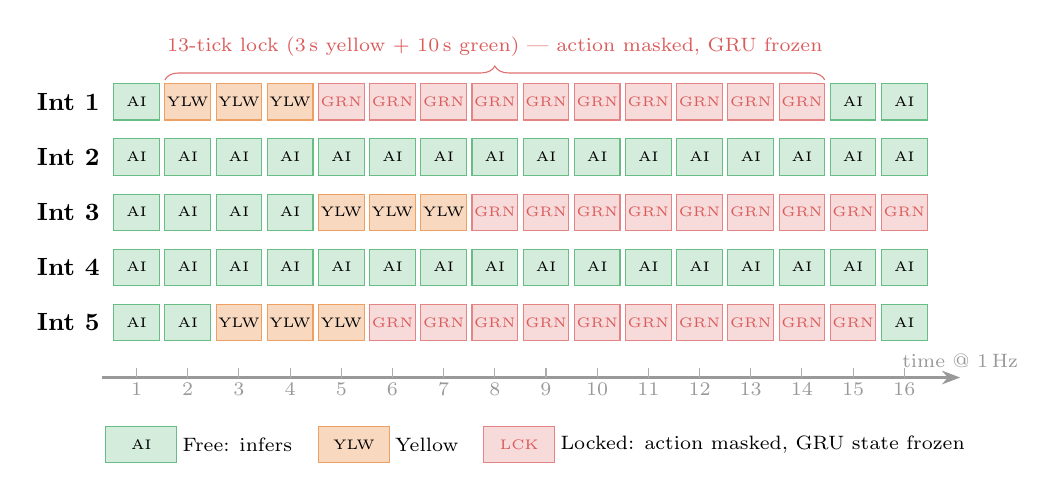
\begin{tikzpicture}[
  font=\small, >=Stealth,
  free/.style={draw=freegreen!70, fill=freegreen!20,
    minimum width=0.58cm, minimum height=0.46cm, inner sep=0pt, font=\tiny},
  ylw/.style={draw=accentorange!70, fill=accentorange!28,
    minimum width=0.58cm, minimum height=0.46cm, inner sep=0pt, font=\tiny},
  lck/.style={draw=lockred!60, fill=lockred!18,
    minimum width=0.58cm, minimum height=0.46cm, inner sep=0pt, font=\tiny},
]
 
% Time header
\foreach \t in {1,...,16}{
  \node[font=\scriptsize, color=gray!80]
    % at ({0.65*\t+0.29}, -3.6) {$t{=}\t$};
    at ({0.65*\t+0.29}, -3.65) {$\t$};
}
 
% Row labels
\node[font=\small\bfseries, right] at (-0.45,  0.0) {Int~1};
\node[font=\small\bfseries, right] at (-0.45, -0.7) {Int~2};
\node[font=\small\bfseries, right] at (-0.45, -1.4) {Int~3};
\node[font=\small\bfseries, right] at (-0.45, -2.1) {Int~4};
\node[font=\small\bfseries, right] at (-0.45, -2.8) {Int~5};
 
%-- ROW 0: Int 1 — switch decided at t=2, lock=13 starts at t=2
%   t=2: YLW (lock=13), t=3: YLW (lock=12), t=4: YLW (lock=11),
%   t=5: GRN transition (lock=10), t=5..14: LCK (lock=9..0), t=15: free
\node[free] at ({0.65*1+0.29},  0.0) {AI};
\node[ylw]  at ({0.65*2+0.29},  0.0) {YLW};
\node[ylw]  at ({0.65*3+0.29},  0.0) {YLW};
\node[ylw]  at ({0.65*4+0.29},  0.0) {YLW};
\foreach \t in {5,...,14}{ \node[lck] at ({0.65*\t+0.29},  0.0) {\tiny\color{lockred!80}GRN}; }
\node[free] at ({0.65*15+0.29}, 0.0) {AI};
\node[free] at ({0.65*16+0.29}, 0.0) {AI};
 
%-- ROW 1: Int 2 — all free
\foreach \t in {1,...,16}{ \node[free] at ({0.65*\t+0.29}, -0.7) {AI}; }
 
%-- ROW 2: Int 3 — switch at t=5, locked t=5..16 (partially visible)
\foreach \t in {1,...,4}{ \node[free] at ({0.65*\t+0.29}, -1.4) {AI}; }
\node[ylw] at ({0.65*5+0.29}, -1.4) {YLW};
\node[ylw] at ({0.65*6+0.29}, -1.4) {YLW};
\node[ylw] at ({0.65*7+0.29}, -1.4) {YLW};
\foreach \t in {8,...,16}{ \node[lck] at ({0.65*\t+0.29}, -1.4) {\tiny\color{lockred!80}GRN}; }
 
%-- ROW 3: Int 4 — all free
\foreach \t in {1,...,16}{ \node[free] at ({0.65*\t+0.29}, -2.1) {AI}; }
 
%-- ROW 4: Int 5 — switch at t=3, locked t=3..15
\node[free] at ({0.65*1+0.29}, -2.8) {AI};
\node[free] at ({0.65*2+0.29}, -2.8) {AI};
\node[ylw]  at ({0.65*3+0.29}, -2.8) {YLW};
\node[ylw]  at ({0.65*4+0.29}, -2.8) {YLW};
\node[ylw]  at ({0.65*5+0.29}, -2.8) {YLW};
\foreach \t in {6,...,15}{ \node[lck] at ({0.65*\t+0.29}, -2.8) {\tiny\color{lockred!80}GRN}; }
\node[free] at ({0.65*16+0.29}, -2.8) {AI};
 
% 1-Hz time axis
\draw[thick, ->, color=gray!80]
  (0.5, -3.5) -- (11.4, -3.5) node[above, font=\scriptsize]{time @ 1\,Hz};
\foreach \t in {1,...,16}{
  \draw[gray!65, thin] ({0.65*\t+0.29}, -3.38) -- ({0.65*\t+0.29}, -3.5);
}
 
% Lock-window brace for Int 1 — includes YLW tick (t=2 through t=14 = 13 ticks)
\draw[decorate, decoration={brace, amplitude=5pt}, color=lockred!70]
  ({0.65*2+0.0}, 0.28) -- ({0.65*14+0.58}, 0.28)
  node[midway, above=5pt, font=\scriptsize, color=lockred!80]
  {13-tick lock (3\,s yellow + 10\,s green) --- action masked, GRU frozen};
 
% Legend
\node[free, minimum width=0.9cm] at (1.0,-4.35) {AI};
\node[right, font=\scriptsize] at (1.40,-4.35) {Free: infers};

\node[ylw,  minimum width=0.9cm] at (3.7,-4.35) {YLW};
\node[right, font=\scriptsize] at (4.10,-4.35) {Yellow};

\node[lck,  minimum width=0.9cm] at (5.8,-4.35) {\tiny\color{lockred!80}LCK};
\node[right, font=\scriptsize] at (6.20,-4.35) {Locked: action masked, GRU state frozen};
 
\end{tikzpicture}
}
    \caption{Asynchronous 1~Hz inference timeline. Each intersection maintains an independent hardware lock counter (13 ticks = 3s yellow + 10s green). Locked intersections have their AI actions masked and GRU states frozen.}
    \label{fig:seq_diag}
    \end{figure}

\subsection{Out-of-Distribution "Gridlock Panic" under Asymmetric Flow}

\paragraph{Challenge} During unidirectional stress tests (e.g., 2,500 vehicles traveling strictly West-to-East), the STGAT agent suffered from Out-of-Distribution (OOD) hallucinations. Because it was trained heavily in symmetric gridlock, the presence of a massive queue triggered a panic, causing the agent to rapidly cycle phases despite the cross-streets being completely empty, effectively halting the major arterial flow. \\
\paragraph{Idea} We introduced a hybrid AI-Hardware \textit{Demand-Responsive Action Mask}. Before the edge device transmits a phase-switch command to the PLC, it queries the red-light approach lanes. If the cross-traffic queue is exactly zero, the hardware vetoes the AI and forces the main street to Rest-in-Green.

    \begin{figure}[H]
    \centering
    % \includegraphics[width=0.6\linewidth]{demand_switch.png}
    \resizebox{0.9\linewidth}{!}{
    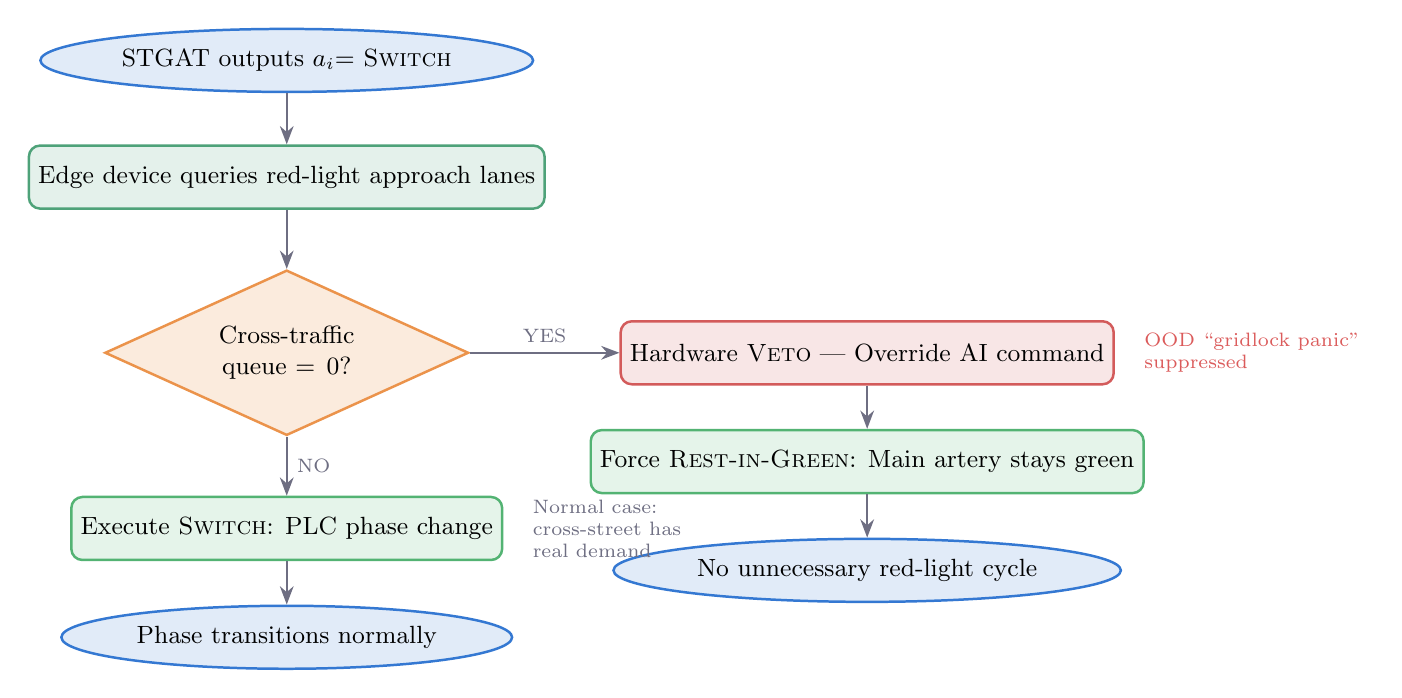
\begin{tikzpicture}[
  font=\small, >=Stealth,
  startend/.style={ellipse, draw=nodeblue, fill=nodeblue!15,
    minimum width=3.2cm, minimum height=0.8cm, line width=0.9pt},
  process/.style={rectangle, rounded corners=4pt,
    draw=layergreen!80, fill=layergreen!12,
    minimum width=3.8cm, minimum height=0.8cm, line width=0.9pt},
  decision/.style={diamond, draw=accentorange!80, fill=accentorange!15,
    minimum width=3.2cm, minimum height=1.2cm, line width=0.9pt,
    aspect=2.2, align=center, text width=2.4cm},
  vetoed/.style={rectangle, rounded corners=4pt,
    draw=accentred!80, fill=accentred!12,
    minimum width=3.8cm, minimum height=0.8cm,
    line width=0.9pt, align=center},
  goact/.style={rectangle, rounded corners=4pt,
    draw=accentgreen!80, fill=accentgreen!12,
    minimum width=3.8cm, minimum height=0.8cm,
    line width=0.9pt, align=center},
  arr/.style={->, thick, color=arrowgray},
]
 
\node[startend]  (start) at (0,0)
  {STGAT outputs $a_i {=}$ \textsc{Switch}};
 
\node[process, below=0.65cm of start] (query)
  {Edge device queries red-light approach lanes};
 
\node[decision, below=0.75cm of query] (check)
  {Cross-traffic queue $= 0$?};
 
% YES → veto branch (right)
\node[vetoed, right=1.9cm of check]   (veto)
  {Hardware \textsc{Veto} --- Override AI command};
\node[goact,  below=0.55cm of veto]   (resting)
  {Force \textsc{Rest-in-Green}: Main artery stays green};
\node[startend, below=0.55cm of resting] (end2)
  {No unnecessary red-light cycle};
 
% NO → proceed branch (down)
\node[goact,    below=0.75cm of check] (exec)
  {Execute \textsc{Switch}: PLC phase change};
\node[startend, below=0.55cm of exec]  (end1)
  {Phase transitions normally};
 
% Arrows
\draw[arr] (start) -- (query);
\draw[arr] (query) -- (check);
\draw[arr] (check) -- node[above, font=\scriptsize]{YES} (veto);
\draw[arr] (check) -- node[right, font=\scriptsize]{NO}  (exec);
\draw[arr] (veto)    -- (resting);
\draw[arr] (resting) -- (end2);
\draw[arr] (exec)    -- (end1);
 
% Side annotations
\node[font=\scriptsize, color=lockred!80, text width=2.8cm, align=left,
      right=0.25cm of veto]
  {OOD ``gridlock panic''\\suppressed};
\node[font=\scriptsize, color=arrowgray, text width=2.8cm, align=left,
      right=0.25cm of exec]
  {Normal case:\\cross-street has\\real demand};
 
\end{tikzpicture}
}
    \caption{Demand-responsive action mask flow. Before executing a phase switch command, the edge device queries red-light approach lanes for halting vehicles. If cross-traffic queue $= 0$, the switch is vetoed and the main artery remains green.}
    \label{fig:demand_switch}
    \end{figure}

\subsection{Topological Blindness in Graph Construction}
\paragraph{Challenge} Real-world SUMO networks (like Patna STC) map single physical roads using dozens of microscopic geometry edges and unsignalized nodes (e.g., yield signs, bends). Initial static Adjacency Matrix formulations only checked one edge deep, failing to realize that two signalized intersections were connected, leaving the GAT layer effectively blind. \\
\paragraph{Proposed idea} The environment's matrix generation was rewritten utilizing a Breadth-First Search (BFS) algorithm. The BFS traverses the physical network, aggregating distances and bypassing unsignalized "dummy" nodes until it strikes the next logical traffic signal, seamlessly collapsing physical geometry into a highly accurate Homogeneous Logical Graph for the attention layer.

\begin{figure}[H]
\centering
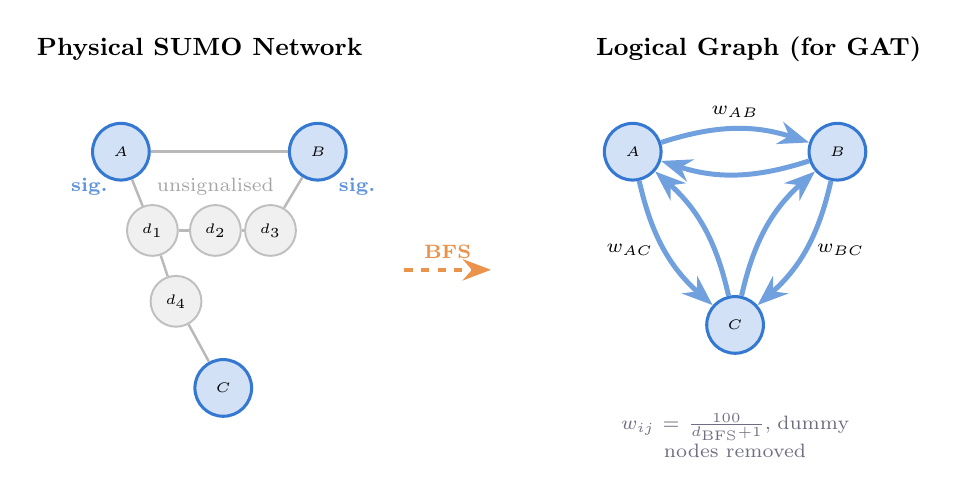
\begin{tikzpicture}[
  font=\small, >=Stealth,
  signode/.style={circle, draw=nodeblue,  fill=nodeblue!22,
                  minimum size=0.72cm, line width=1.1pt},
  dummy/.style  ={circle, draw=gray!50,  fill=gray!12,
                  minimum size=0.42cm, line width=0.7pt},
  pe/.style={draw=gray!55, line width=0.9pt},
  le/.style={draw=nodeblue!70, line width=1.8pt, ->, >=Stealth},
  bfs/.style={->, very thick, color=accentorange!80, dashed},
]
 
%-- LEFT: Physical SUMO topology
\node[font=\bfseries\small] at (-4.5, 2.3) {Physical SUMO Network};
 
\node[signode] (A) at (-5.5, 1.0) {\tiny$A$};
\node[signode] (B) at (-3.0, 1.0) {\tiny$B$};
\node[dummy]   (d1) at (-5.1, 0.0) {\tiny$d_1$};
\node[dummy]   (d2) at (-4.3, 0.0) {\tiny$d_2$};
\node[dummy]   (d3) at (-3.6, 0.0) {\tiny$d_3$};
\node[dummy]   (d4) at (-4.8,-0.9) {\tiny$d_4$};
\node[signode] (C) at (-4.2,-2.0) {\tiny$C$};
 
\draw[pe] (A)--(d1); \draw[pe] (d1)--(d2);
\draw[pe] (d2)--(d3); \draw[pe] (d3)--(B);
\draw[pe] (d1)--(d4); \draw[pe] (d4)--(C);
\draw[pe] (A)--(B);
 
\node[font=\scriptsize, color=gray!70]     at (-4.3, 0.55) {unsignalised};
\node[font=\scriptsize, color=nodeblue!80] at (-5.9, 0.55) {\bfseries sig.};
\node[font=\scriptsize, color=nodeblue!80] at (-2.5, 0.55) {\bfseries sig.};
 
%-- Arrow
\draw[bfs, line width=1.6pt]
  (-1.9,-0.5) -- node[above, font=\scriptsize\bfseries]{BFS} (-0.8,-0.5);
 
%-- RIGHT: Logical graph
\node[font=\bfseries\small] at (2.6, 2.3) {Logical Graph (for GAT)};
 
\node[signode] (LA) at (1.0, 1.0) {\tiny$A$};
\node[signode] (LB) at (3.6, 1.0) {\tiny$B$};
\node[signode] (LC) at (2.3,-1.2) {\tiny$C$};
 
\draw[le, bend left=18]  (LA) to node[above, font=\scriptsize]{$w_{AB}$} (LB);
\draw[le, bend left=18]  (LB) to (LA);
\draw[le, bend right=18] (LA) to node[left,  font=\scriptsize]{$w_{AC}$} (LC);
\draw[le, bend right=18] (LC) to (LA);
\draw[le, bend left=18]  (LB) to node[right, font=\scriptsize]{$w_{BC}$} (LC);
\draw[le, bend left=18]  (LC) to (LB);
 
\node[font=\scriptsize, color=arrowgray, text width=3.2cm, align=center]
  at (2.3,-2.6) {$w_{ij}=\tfrac{100}{d_\mathrm{BFS}+1}$,\;dummy nodes removed};
 
\end{tikzpicture}
\caption{BFS-based logical graph construction. Unsignalised dummy nodes
(yield signs, geometry bends) are skipped; road distances are accumulated
to yield a compact homogeneous graph over the $N{=}10$ signalised intersections.}
\label{fig:bfs_graph}
\end{figure}

\subsection{Fair Comparative Benchmarking}
\paragraph{Challenge} Initial comparison charts between the Baseline and Agent showed immense, inexplicable variance. Investigation revealed differing mathematical standards: the RL agent used scaled tensor arrays, while the baseline read raw TraCI integer metrics. Moreover, differing SUMO random seeds generated completely separate traffic scenarios. \\
\paragraph{Proposed idea} We enforced a strict deterministic seed passed directly from the React UI to both Python runners. All normalizations were unified, ensuring the Baseline runner evaluates identical demand traffic geometries.

\subsection{WebSocket ASGI Concurrency}
\paragraph{Challenge} As episodes began, the React UI re-renders repeatedly severed the WebSocket connection, causing fatal \texttt{Unexpected ASGI message} runtime exceptions on the backend when it attempted to stream step-data. \\
\paragraph{Proposed idea} State management was decoupled using static \texttt{useRef} hooks to track \texttt{run\_id}s without destroying and rebuilding the websocket tree mid-cycle.

\section{Hardware and Software Specifications}
\subsection{Physical Deployment Stack}
\begin{itemize}
    \item \textbf{Visual Sensing \& Perception:} Pole-mounted 1080p IP Cameras running YOLOv8/v9 object detection for real-time PCU mapping and queue length extraction.
    \item \textbf{Fog Compute Node:} NVIDIA Jetson AGX Orin or a centralized Local Data Center Server running Ubuntu 22.04 LTS to handle simultaneous multi-intersection STGAT inference.
    \item \textbf{PLC Interface:} NTCIP compliant traffic controller hardware for executing physical phase shifts.
    \item \textbf{Telemetry Backbone:} 4G/5G cellular modems running MQTT over TLS 1.2 for secure, low-latency telemetry transmission from Edge to Fog to Cloud.
\end{itemize}

\subsection{Simulation and Development Stack}
\begin{itemize}
    \item \textbf{Traffic Simulator:} Eclipse SUMO $\geq$ 1.18.0. Training uses \texttt{libsumo} (in-process) for speed, while inference uses \texttt{traci} (subprocess mode) mapped to SUMO-GUI.
    \item \textbf{Deep Learning Backend:} Python 3.10+, PyTorch 2.0+ (CUDA), FastAPI, Uvicorn (ASGI) for asynchronous WebSocket handling.
    \item \textbf{Training Hardware:} Dedicated NVIDIA RTX 3060 12GB (or equivalent) minimum.
    \item \textbf{IoT Microservices:} Eclipse Mosquitto 2.0+ (MQTT Broker), InfluxDB 2.x (Time-Series DB), Docker Compose for container orchestration.
    \item \textbf{Frontend \& Rendering:} Node.js 18+, React (Vite.js) with Recharts for 2D metrics, and \textbf{Unity 3D Engine} for live photorealistic spatial rendering.
\end{itemize}
\section{Conclusion}
The fusion of Graph Attention Networks with Proximal Policy Optimization directly addresses the failures of isolated and pre-timed traffic control paradigms. By introducing $K{=}3$ hop spatial awareness across 10 signalized intersections, the STGAT model successfully prevents ripple-effect gridlocks that plague both Independent Q-Learning and fixed-timing baselines. The demand-responsive action mask further stabilizes the agent against out-of-distribution traffic patterns.

The engineering contributions are equally significant: asynchronous 1~Hz hardware locks decouple intersection control from global simulation stepping, BFS-based adjacency construction handles complex real-world SUMO topologies, and deterministic seeding ensures fair benchmarking against baseline controllers.

Paired with a robust microservice IoT architecture---featuring MQTT telemetry, InfluxDB time-series persistence, WebSocket streaming, and a real-time React monitoring dashboard---this work provides a transparent, scalable bridge between academic Deep Reinforcement Learning models and production-ready Smart City deployments.

\section{Future Work}
Several directions remain for extending this architecture:

\subsection{Model Quantization for Edge Deployment}
The current STGAT model operates in FP32 precision. For deployment on power-constrained edge devices (Jetson Orin Nano, 15W), the model should be quantized to INT8 using NVIDIA TensorRT or PyTorch's built-in quantization toolkit. This would reduce inference latency from $\sim$8ms to $<$1ms and cut memory footprint by $4\times$, enabling multi-intersection inference on a single edge node.

\subsection{Camera-Based Perception Integration}
The current system assumes TraCI provides perfect vehicle state information. In physical deployment, perception noise from camera-based detection (YOLOv8/v9) will introduce uncertainty in PCU counts and queue measurements. Future work should:
\begin{itemize}
    \item Train the STGAT agent with \textit{observation noise injection} (Gaussian noise on $q_i$ and $w_i$) during simulation to build robustness.
    \item Implement a Kalman filter or Bayesian fusion layer between the YOLO detector output and the GNN input tensor.
\end{itemize}

\subsection{Multi-Objective Reward Shaping}
The current reward $r_i = -(q_i + 0.5 w_i) - 15 \cdot \mathbb{1}[\text{switch}]$ treats all vehicle types equally. Future formulations could incorporate:
\begin{equation}
    r_i^{(t)} = -\left( q_i + \omega w_i + \beta \cdot \text{CO}_2(i,t) + \gamma \cdot d_{\text{emergency}}(i,t) \right)
\end{equation}
where $\text{CO}_2$ penalizes idle emissions (proportional to PCU-weighted queue $\times$ time) and $d_{\text{emergency}}$ provides priority preemption for ambulances/fire trucks detected via V2X or YOLO classification.

\subsection{Federated Learning across Cities}
The current model is trained centrally on one city topology. Federated Learning could enable multiple cities to collaboratively improve a shared STGAT backbone without exchanging raw traffic data---only gradient updates---addressing both data privacy and domain generalization.

\subsection{Cloud-Native Scaling}
Transitioning from local Docker Compose to managed cloud services:
\begin{itemize}
    \item \textbf{MQTT:} AWS IoT Core or Azure IoT Hub for managed broker with TLS mutual authentication.
    \item \textbf{TSDB:} Amazon Timestream or InfluxDB Cloud for auto-scaling time-series storage.
    \item \textbf{Inference:} AWS Lambda@Edge or Azure IoT Edge for serverless model serving.
\end{itemize}
\section*{Author Contributions}
This project was conceptualized, engineered, and evaluated collaboratively by Team D3SR (IIT ISM Dhanbad). Primary individual contributions are outlined as follows:
\begin{itemize}
    \item \textbf{Divya Prakash Sinha:} Primary architect of the STGAT reinforcement learning model. Formulated the GNN spatial embedding pipeline, multi-head attention logic, and PPO critic thresholds. Conducted the baseline algorithm ablation mathematics and reward function engineering.
    \item \textbf{Dyuti Ballav Paul:} Lead simulation engineer for the Eclipse SUMO Digital Twin. Mapped the physical Patna STC road networks into the TraCI environment, managed the BFS-based graph adjacency geometry, and engineered the critical asynchronous 1~Hz hardware locking mechanism.
    \item \textbf{Devansh Gupta:} Engineered the Cloud Backend API infrastructure. Developed the FastAPI WebSocket asynchronous data-streaming pipelines and integrated the InfluxDB time-series database for historical RL telemetry persistence.
    \item \textbf{Shreyas Kumar Patel:} Lead Frontend and Rendering developer. Designed and built the React/Vite Dashboard with real-time Recharts datastreams, and integrated the \textbf{Unity 3D Engine} to deliver a fully immersive, photorealistic Digital Twin of the traffic environment.
    \item \textbf{Rishit Das:} Edge and IoT Protocols engineer. Orchestrated the Mosquitto MQTT message brokering between the inference endpoints and backend, and authored the physical deployment topology for NVIDIA Jetson nodes and automated camera integration.
\end{itemize}

\appendices
\section{Live Dashboards and Digital Twins}
The theoretical architectures proposed in this paper have been fully translated into the live monitoring interfaces demonstrated below.

\begin{figure}[H]
    \centering
    % UNCOMMENT THE LINE BELOW AND REPLACE WITH YOUR ACTUAL FILE NAME
    % \includegraphics[width=0.96\linewidth]{unity_twin.png} 
    \caption{The Unity 3D Digital Twin rendering the physical Patna STC environment, ingesting real-time metrics and phase states from the cloud backend.}
    \label{fig:app_unity}
\end{figure}

\begin{figure}[H]
    \centering
    % UNCOMMENT THE LINE BELOW AND REPLACE WITH YOUR ACTUAL FILE NAME
    % \includegraphics[width=0.96\linewidth]{dashboard.png} 
    \caption{The React/Vite-based Dashboard visualizing real-time WebSocket telemetry, streaming intersection wait-times, and aggregated model performance analytics.}
    \label{fig:app_dash}
\end{figure}

\begin{thebibliography}{00}
\bibitem{b1} Krajzewicz, D., Erdmann, J., Behrisch, M., and Bieker, L., ``Recent Development and Applications of SUMO - Simulation of Urban MObility,'' \textit{Int'l Journal On Advances in Systems and Measurements}, vol. 5, no. 3\&4, pp. 128--138, 2012.
\bibitem{b2} Schulman, J., Wolski, F., Dhariwal, P., Radford, A., and Klimov, O., ``Proximal Policy Optimization Algorithms,'' \textit{arXiv preprint arXiv:1707.06347}, 2017.
\bibitem{b3} Velickovic, P., Cucurull, G., Casanova, A., Romero, A., Lio, P., and Bengio, Y., ``Graph Attention Networks,'' \textit{ICLR}, 2018.
\bibitem{b4} Zhang, Y., Yu, Z., Zhang, J., Wang, L., Luan, T. H., Guo, B., and Yuen, C., ``Learning Decentralized Traffic Signal Controllers with Multi-Agent Graph Reinforcement Learning,'' \textit{arXiv preprint arXiv:2311.03756}, 2023.
\end{thebibliography}

\end{document}
